%==============================================================================
% Sjabloon poster bachproef
%==============================================================================
% Gebaseerd op document class `a0poster' door Gerlinde Kettl en Matthias Weiser
% Aangepast voor gebruik aan HOGENT door Jens Buysse en Bert Van Vreckem

\documentclass[a0,portrait]{hogent-poster}

\usepackage{xcolor}
\usepackage{caption}
\usepackage{wrapfig}

% Info over de opleiding
\course{Bachelorproef}
\studyprogramme{toegepaste informatica}
\academicyear{2025-2026}
\institution{Hogeschool Gent, Valentin Vaerwyckweg 1, 9000 Gent}

% Info over de bachelorproef
\title{Ondersteuning van energieplanning via GIS: ontwerp en implementatie van een analysetool voor de Einstein Telescoop}
% \subtitle{Ondertitel (eventueel)}
\author{Andries\ Ulenaers}
\email{andries.ulenaers@student.hogent.be}
\supervisor{V.\ Depestele} 
\cosupervisor{Prof.\ dr.\ B.\ Vermang\ (EnergyVille/UHasselt)}

% Indien ingevuld, wordt deze informatie toegevoegd aan het einde van de
% abstract. Zet in commentaar als je dit niet wilt.
\specialisation{Softwareontwikkeling}
\keywords{Lambda-calculus, Scheme}
\projectrepo{https://github.com/Andries-U/BP_Andries-Ulenaers_2025-2026}
\date{\today}

\begin{document}

\maketitle

% \begin{abstract}
% Deze bachelorproef onderzoekt hoe een GIS-gebaseerde tool kan bijdragen aan de energieplanning voor de \textbf{Einstein Telescoop (ET)}, een geplande zwaartekrachtgolfdetector in de \textbf{Euregio Maas-Rijn (EMR)}. De ET stelt hoge eisen aan energievoorziening: betrouwbaarheid, trillingsvrijheid, en duurzaamheid, met aandacht voor lokale maatschappelijke draagkracht en innovatieve hernieuwbare bronnen zoals \textbf{Agro-Photovoltaics (AgriPV)}. De tool analyseert geografische datasets om potentiële locaties voor energie-infrastructuur te identificeren, rekening houdend met ecologische beperkingen (bv. Natura2000-gebieden) en grensoverschrijdende data.
% \end{abstract}

{\color{black}\hrule height 1pt width \hsize}

\begin{multicols}{2}
\section{Inleiding}

\noindent
\begin{minipage}[t]{0.62\columnwidth}

De \textbf{Einstein Telescope (ET)} is een toekomstige, ultragevoelige zwaartekrachtgolfdetector die mogelijk in de Euregio Maas-Rijn (EMR) (Figuur~\ref{fig:einstein-telescope}) wordt gebouwd. Het gebruik van de telescoop vereist \textbf{veel energie}. Ook stelt de onderzoeksgroep hoge eisen aan \textbf{betrouwbaarheid}, \textbf{duurzaamheid} en \textbf{trillingsvrijheid}.

In dit onderzoek wordt een \textbf{GIS-analysetool} ontwikkeld die onderzoekers ondersteunt bij het \textbf{analyseren} van \textbf{geografische data}, zoals landbouwgebieden, stortplaatsen en waterlichamen. Hierdoor kunnen onderzoekers snel en nauwkeurig bepalen waar en hoeveel \textbf{capaciteit} voor duurzame \textbf{energiebronnen} beschikbaar is, bijvoorbeeld voor zonnepanelen op landbouwgrond of wateroppervlakken.

\end{minipage}\hfill
\begin{minipage}[t]{0.32\columnwidth}
    \vspace{0pt}
    \centering
    \includegraphics[width=\linewidth]{../graphics/Tool/search-area_20260523_v2.png}
    \captionof{figure}{Voorgesteld zoekgebied (lichtblauw) voor de locatie van de ET in de EMR}\label{fig:einstein-telescope}
\end{minipage}

\section{Achtergrond}

% De Einstein Telescope zal een grote impact hebben, zowel wetenschappelijk als regionaal. Op wetenschappelijk vlak biedt het project nieuwe inzichten in zwaartekrachtgolven, fundamentele natuurkunde en gerelateerde technologische ontwikkelingen. Voor de Euregio Maas-Rijn brengt de komst van de Einstein Telescope onder andere de volgende voordelen met zich mee:

% \begin{itemize}
%     \item \textbf{Economische groei}: jobcreatie en technologische innovatie.
%     \item \textbf{Maatschappelijke impact}: meer bedrijvigheid in stille landerlijke regio.
% \end{itemize}
\begin{wrapfigure}{r}{0.25\textwidth}
    \centering
    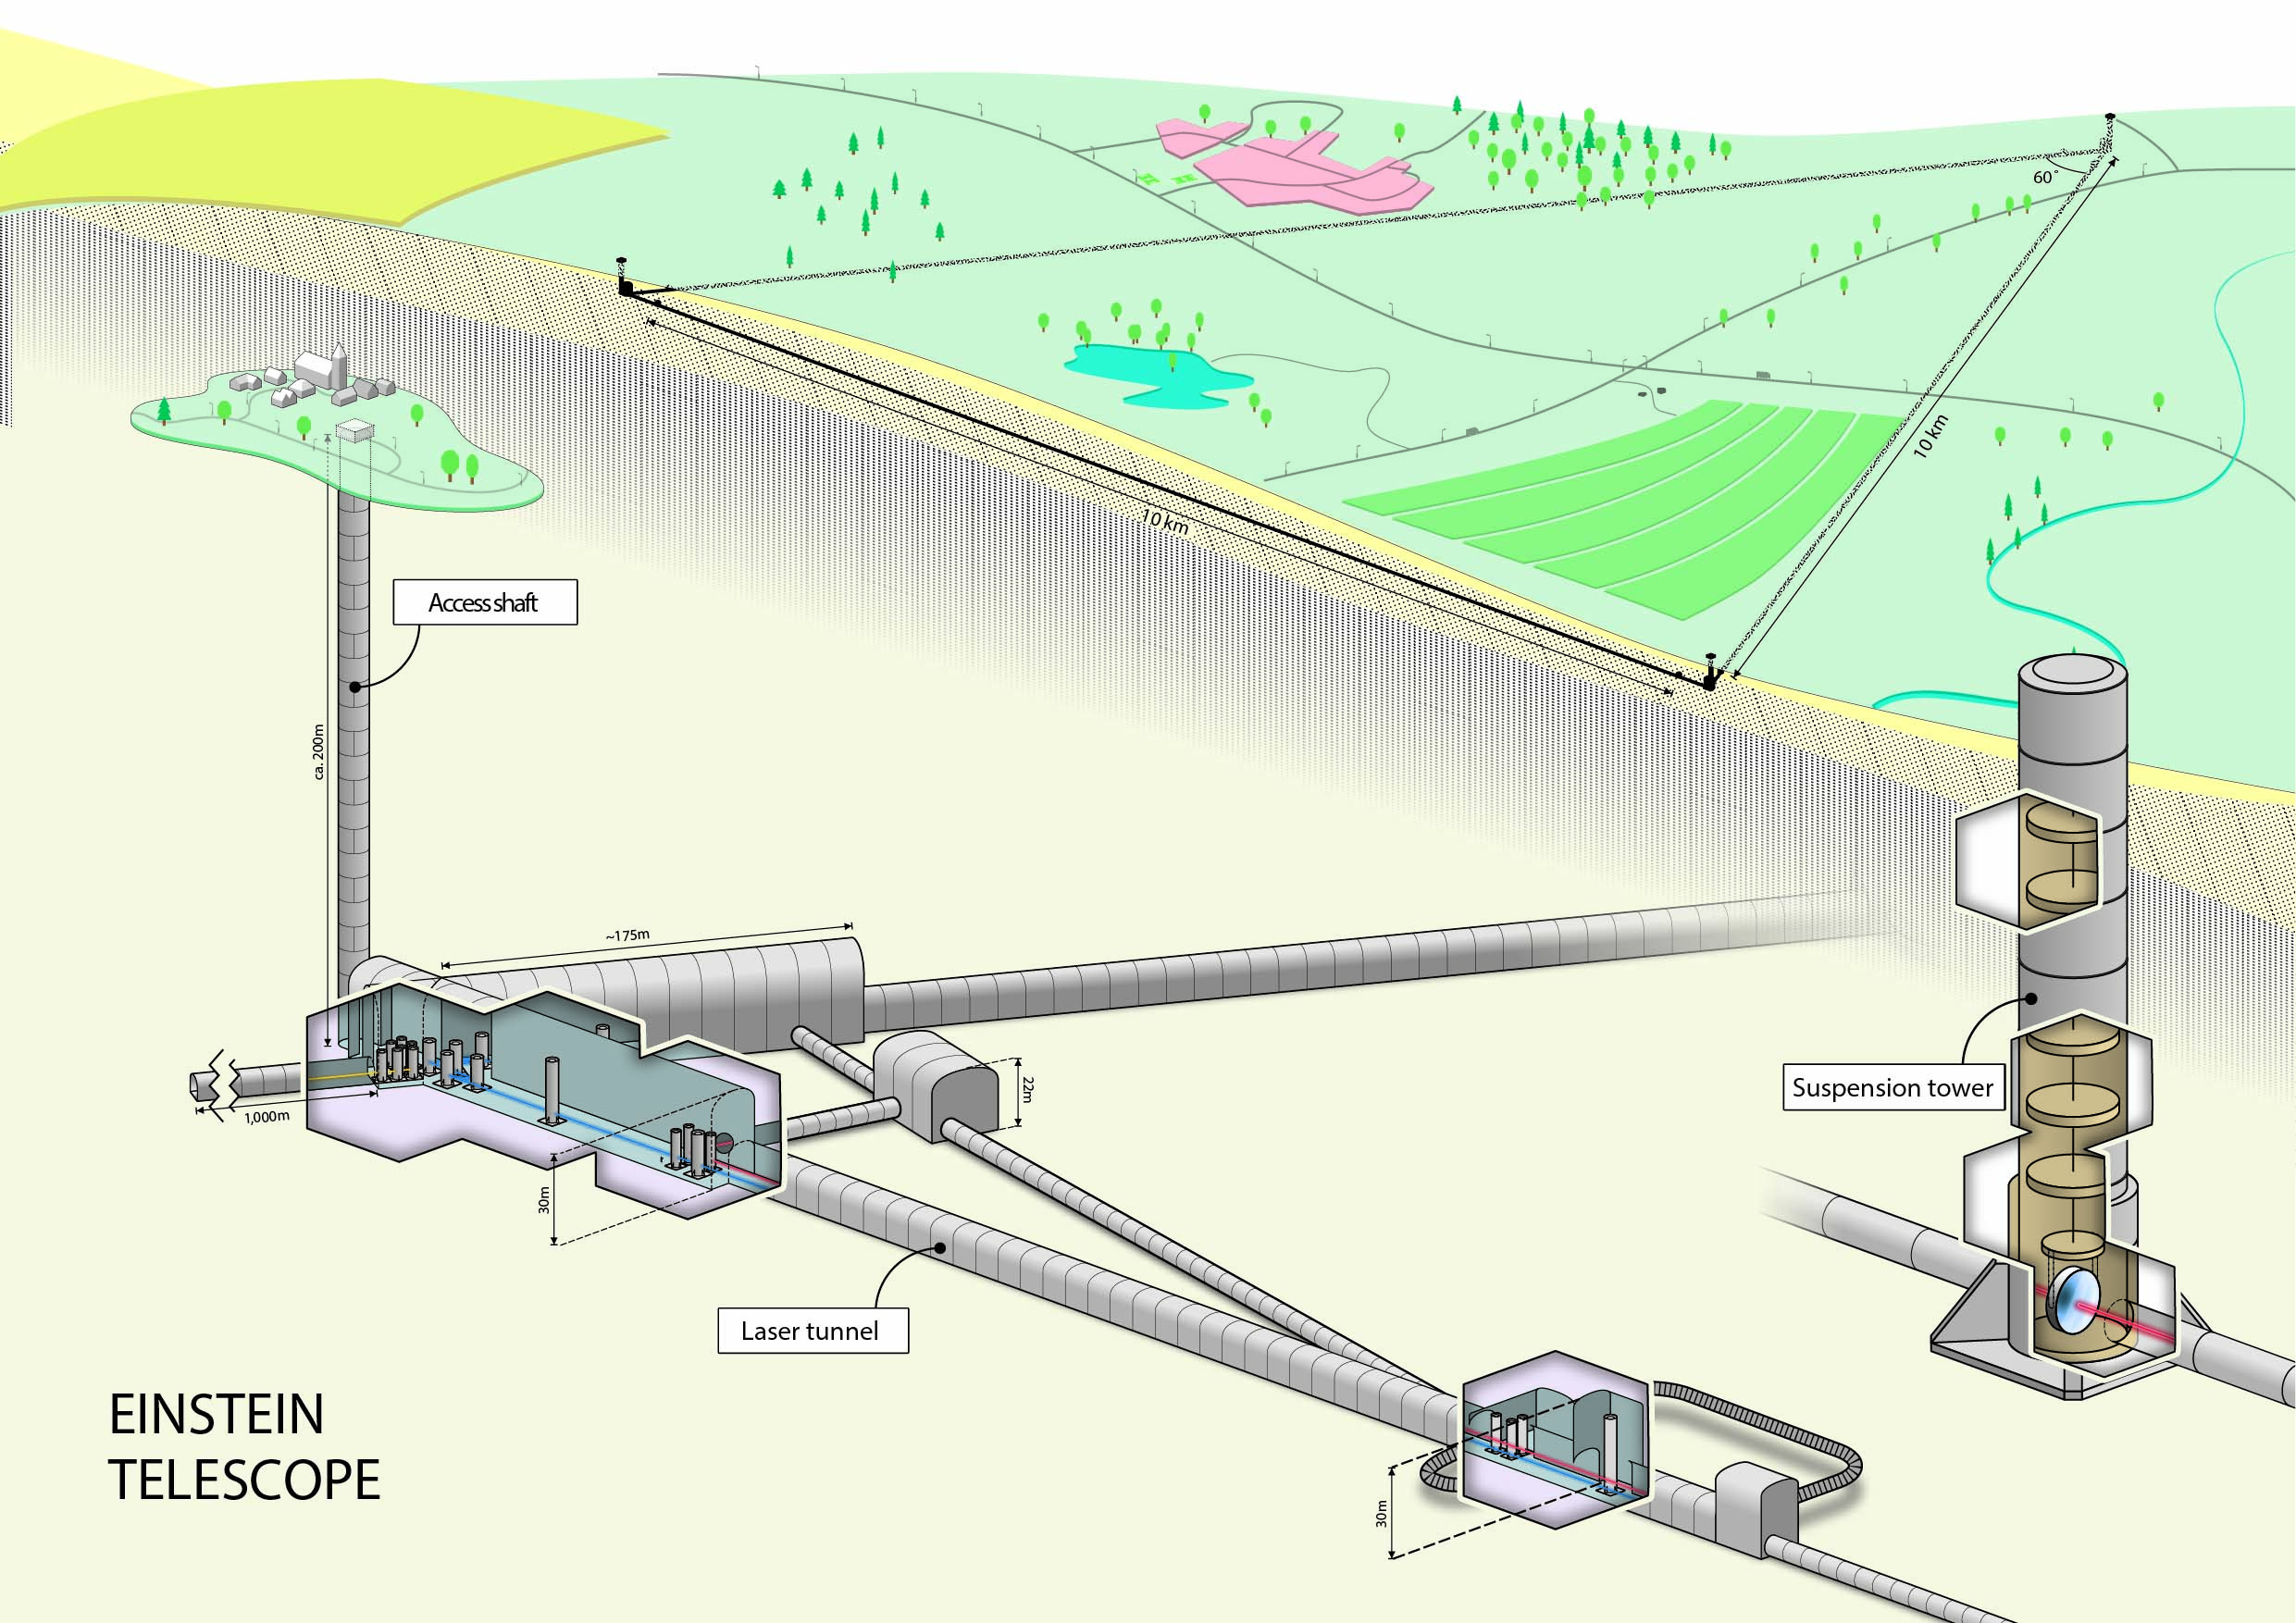
\includegraphics[width=\linewidth]{../graphics/Einstein_Telescope/einstein_telescope_ALT-EN-01_web.png}
    \captionof{figure}{Illustratieve voorstelling van de Einstein Telescope ©T. Balder/Nikhef}
\end{wrapfigure}


De Einstein Telescope zal een grote impact hebben:

\begin{itemize}
    \item \textcolor{hogent-darkgreen}{\textbf{Wetenschappelijk}}:
    \begin{itemize}
        \item nieuwe inzichten in \textbf{zwaartekrachtgolven}.
        \item beter begrip \textbf{fundamentele natuurkunde}
        \item andere gerelateerde en ongerelateerde \textbf{technologische ontwikkelingen}
    \end{itemize}
    \item \textcolor{hogent-pink}{\textbf{Regionaal}}:
    \begin{itemize}
        \item \textbf{Economische groei}: jobcreatie en technologische innovatie
        \item \textbf{Maatschappelijke impact}: meer bedrijvigheid in een stille landerlijke regio
    \end{itemize}
\end{itemize}
\medskip

Om de Einstein Telescope naar de EMR-regio te halen, moet een haalbaar energie\-plan worden voorgelegd. Dit plan moet rekening houden met verschillende aspecten:
\begin{itemize}
    \item \textcolor{hogent-ochre}{\textbf{Technische eisen}}: trillingsvrije en duurzame energie.
    \item \textcolor{hogent-purple}{\textbf{Ecologische beperkingen}}: Natura 2000-gebieden en verantwoord landgebruik.
    \item \textcolor{hogent-lightgreen}{\textbf{Maatschappelijke wensen}}: lokale betrokkenheid en innovatieve oplossingen.
\end{itemize}

\section{Methode}

Voor de ontwikkeling van de analysetool werden vier fasen doorlopen:

\begin{enumerate}
    \item \textcolor{hogent-brown}{\textbf{Vereistenanalyse}}: identificatie van behoeften onderzoekers en benodigde datasets.
    
    \item \textcolor{hogent-grey}{\textbf{Vergelijking van GIS-tools}}: evalueren geschiktheid GIS-oplossingen.
    
    \item \textcolor{hogent-yellow}{\textbf{Ontwikkeling van een proof-of-concept}}:
    % \begin{itemize}
    %     \item \textbf{Genereren} hoekpunten van de Einstein Telescope.
    %     \item \textbf{Filteren} van datasets op basis van onderzoeksgebied en gebruikersvereisten.
    %     \item \textbf{Visualiseren} en \textbf{exporteren} van resultaten.
    % \end{itemize}
    
    \item \textcolor{hogent-orange}{\textbf{Risicoanalyse}}: identificatie van beperkingen en risico's
\end{enumerate}


\section{Resultaten}


\begin{enumerate}
    \item \textbf{Selectie QGIS} als basis: open-source, krachtige GIS-functionaliteiten, en uitgebreide Python-integratie.
    \item \textbf{Proof-of-concept} tool ontwikkeld met functionaliteiten voor:
    \begin{itemize}
        \item \textbf{Genereren zoekgebied} met instelbare straal rond hoekpunten van de ET.\@
        \item \textbf{Berekenen oppervlakte} van percelen binnen het zoekgebied.
         \item \textbf{Volledige analyse}: geeft een overzicht van alle categorieën binnen een dataset, inclusief oppervlakte per categorie. Ideaal om een \textbf{algemeen beeld} van de dataset en mogelijkheden te krijgen.
        \item \textbf{Gedeeltelijke analyse}: filtert de dataset op \textbf{specifieke waarden}, zoals landbouwpercelen met een bepaald type teelt. Ideaal om gericht te zoeken naar specifieke locaties.
        \item \textbf{Export analyseresultaten} via:
            \begin{itemize}
                \item \textbf{PDF-rapporten} met kaarten en tabellen, 
                \item \textbf{QGIS-datalagen} 
                \item \textbf{CSV-bestanden} met ruwe data.
            \end{itemize}
    \end{itemize}
    \item \textbf{Identificatie beperkingen en risico's} zoals dubbele telling en beperkingen door datakwaliteit

\end{enumerate}

% De proof-of-concept tool heeft twee types van analyses:
% \begin{itemize}
%     \item \textbf{Volledige analyse}: geeft een overzicht van alle categorieën binnen een dataset, inclusief oppervlakte per categorie. Ideaal om een algemeen beeld van de dataset en mogelijkheden te krijgen.
%     \item \textbf{Gedeeltelijke analyse}: filtert de dataset op specifieke waarden, zoals landbouwpercelen met een bepaald type teelt. Ideaal om gericht te zoeken naar specifieke locaties.
% \end{itemize}

\begin{center}
    \begin{minipage}{0.45\linewidth}
        \centering
        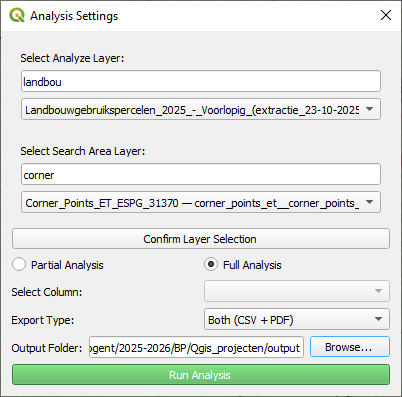
\includegraphics[width=\linewidth]{../graphics/Tool/gui-screen_volledige-analyse_V2.png}
        \captionof{figure}{Illustratieve voorstelling van de Einstein Telescope ©T. Balder/Nikhef}
    \end{minipage}%
    \hspace{1cm}
    \begin{minipage}{0.45\linewidth}
        \centering
        \includegraphics[width=\linewidth]{../graphics/Tool/maps_after_analyze.png}
        \captionof{figure}{Illustratieve voorstelling van de Einstein Telescope ©T. Balder/Nikhef}
    \end{minipage}
\end{center}


\section{Conclusie}

Dit onderzoek toont aan dat open-source GIS-tools zoals QGIS, gecombineerd met Python, krachtige oplossingen kunnen bieden voor complexe specifieke ruimtelijke vraagstukken. De ontwikkelde tool:

\begin{itemize}
    \item ondersteunt Einstein Telescope-onderzoekers bij het identificeren van geschikte locaties voor duurzame energieproductie;
    \item maakt geografische analyses toegankelijk voor gebruikers met beperkte GIS expertise.
    \item vormt een basis voor mogelijke toekomstige uitbreidingen
    \begin{itemize}
        \item Integratie van \textbf{energiepotentieelberekeningen}
        \item Implementatie van \textbf{multi-criteria-analyses} waarin objectieve gegevens met subjectieve criteria afwegen
    \end{itemize}
\end{itemize}



% Tijdens het onderzoek werden bovendien enkele belangrijke inzichten opgedaan:

% \begin{itemize}
%     \item Samenwerking met stakeholders, waaronder onderzoekers en overheden, is essentieel voor een succesvol resultaat.
%     \item Flexibiliteit in de software is noodzakelijk omdat vereisten tijdens het project kunnen evolueren.
%     \item Het expliciet benoemen van beperkingen en risico's, zoals datakwaliteit en mogelijke dubbele tellingen, is belangrijk voor realistische verwachtingen en correcte interpretatie van resultaten.
% \end{itemize}

\end{multicols}


\end{document}




% % =============================================================================
% % Origineel voorbeeldposter
% % =============================================================================
% \begin{document}
% \maketitle

% \begin{abstract}
% It's only a model.
% You don't vote for kings. Who's that then? We found them. Ni! Ni! Ni! Ni!
% The nose? On second thoughts, let's not go there. It is a silly place. Bloody Peasant! And the hat. She's a witch! Where'd you get the coconuts?
% \end{abstract}

% \begin{multicols}{2} % This is how many columns your poster will be broken into, a portrait poster is generally split into 2 columns

% \section{Introductie}

% Be quiet! Found them? In Mercia?! The coconut's tropical! But you are dressed as one… Well, what do you want? Knights of Ni, we are but simple travelers who seek the enchanter who lives beyond these woods.

% Well, what do you want? It's only a model. Camelot! We found them. We shall say `Ni' again to you, if you do not appease us.

% The nose? Shut up! Burn her! I am your king. You don't vote for kings.

% You can't expect to wield supreme power just `cause some watery tart threw a sword at you! Well, we did do the nose. I don't want to talk to you no more, you empty-headed animal food trough water! I fart in your general direction! Your mother was a hamster and your father smelt of elderberries! Now leave before I am forced to taunt you a second time!

% Why do you think that she is a witch? We want a shrubbery!! I don't want to talk to you no more, you empty-headed animal food trough water! I fart in your general direction! Your mother was a hamster and your father smelt of elderberries! Now leave before I am forced to taunt you a second time!

% \section{Experimenten}

% A newt? Camelot! Why? No, no, no! Yes, yes. A bit. But she's got a wart.

% Shut up! I dunno. Must be a king. Who's that then? Look, my liege! On second thoughts, let's not go there. It is a silly place.

% Shut up! Will you shut up?! No, no, no! Yes, yes. A bit. But she's got a wart. He hasn't got shit all over him. It's only a model. It's only a model.

% Bring her forward! I don't want to talk to you no more, you empty-headed animal food trough water! I fart in your general direction! Your mother was a hamster and your father smelt of elderberries! Now leave 

% \section{Sectie met figuur}

% De {\LaTeX} figure-omgeving bepaalt zelf waar een afbeelding komt en dat is meestal niet op de plek in de tekst waar de figure-omgeving gedefinieerd wordt. Als je wilt forceren dat afbeeldingen toch in de flow van de tekst blijven, dan kan je dat zoals hieronder:

% \begin{center}
%   \captionsetup{type=figure}
%   
\includegraphics[width=1.0\linewidth]{grail}
%   \captionof{figure}{He hasn't got shit all over him. The nose? Where'd you get the coconuts? What do you mean? We shall say `Ni' again to you, if you do not appease us}
% \end{center}

% Let er wel op dat dit tot problemen met bladschikking kan leiden.

% \section{Conclusies}

% Don't underestimate the Force. Oh God, my uncle. How am I ever gonna explain this? I suggest you try it again, Luke. This time, let go your conscious self and act on instinct. Don't be too proud of this technological terror you've constructed. The ability to destroy a planet is insignificant next to the power of the Force.

% \section{Toekomstig onderzoek}

% I care. So, what do you think of her, Han? No! Alderaan is peaceful. We have no weapons. You can't possibly… I have traced the Rebel spies to her. Now she is my only link to finding their secret base.

% Kid, I've flown from one side of this galaxy to the other. I've seen a lot of strange stuff, but I've never seen anything to make me believe there's one all-powerful Force controlling everything. There's no mystical energy field that controls my destiny. It's all a lot of simple tricks and nonsense. You are a part of the Rebel Alliance and a traitor! Take her away! 

% \end{multicols}
% \end{document}